%!TEX program = lualatex
\documentclass[a4paper,12pt]{article}

% ===== Idioma =====
\usepackage[portuguese]{babel}
\addto\captionsportuguese{%
  \renewcommand{\contentsname}{Sumário}%
  \renewcommand{\listfigurename}{Lista de Figuras}%
  \renewcommand{\listtablename}{Lista de Tabelas}%
}

% ===== Fonte (LuaLaTeX) =====
\usepackage{fontspec}
\setmainfont{Latin Modern Roman}

% ===== Layout =====
\usepackage[top=3cm,bottom=2cm,left=3cm,right=2cm]{geometry}
\usepackage{indentfirst}
\usepackage{setspace}
\onehalfspacing
\setlength{\parindent}{1.25cm}
\setlength{\parskip}{0pt}

% ===== Tabelas / listas =====
\usepackage{booktabs}
\usepackage{enumitem}
\setlist[itemize]{noitemsep,topsep=3pt}

% ===== Figuras gerais =====
\usepackage{graphicx}
\usepackage{float}
\usepackage{pdflscape}
\graphicspath{{./}{./imagens/}{./figuras/}{./Figs/}}

% ===== Links =====
\usepackage[hidelinks]{hyperref}
\usepackage{xurl}
\Urlmuskip=0mu plus 1mu

% ===== Bibliografia =====
\usepackage{csquotes}
\usepackage[
  backend=biber,
  style=abnt,
  sorting=nyt
]{biblatex}
\addbibresource{tcc_desc.bib}

% ===== TikZ (fluxogramas/diagramas) =====
\usepackage[dvipsnames]{xcolor}
\usepackage{tikz}
\usetikzlibrary{shapes.geometric, arrows.meta, positioning}
% \input{flu1_styles}

% ===== Química =====
\usepackage[version=4]{mhchem}
%====================
% Unidades
%===================
\usepackage{siunitx}

\begin{document}

% ================== FOLHA DE ROSTO ==================
\begin{titlepage}
  \begin{center}
    \vspace*{-1cm}
    
\includegraphics[width=3cm]{D:/LaTex_Projects/Projetos_Latex/Descomissionamento/uerj.jpg}\\[0.8cm]

    \textbf{UNIVERSIDADE DO ESTADO DO RIO DE JANEIRO}\\[0.2cm]
    \textbf{FACULDADE DE OCEANOGRAFIA}\\[0.2cm]

    \textbf{Proposta de estudo para TCC}\\[0.5cm]
    \textbf{Descomissionamento de UEPs e sistemas Subsea de Produção.}\\[8cm]
  \end{center}

  \vfill

  \begin{flushright}
    Aluno: José Mauro Xavier Elsas\par
    Disciplina: Oceanografia\par
    Professor: David Zee
  \end{flushright}

  \vfill

  \begin{center}
    Rio de Janeiro\\
    Janeiro de 2026
  \end{center}
\end{titlepage}

\tableofcontents
\newpage

\phantomsection
\addcontentsline{toc}{section}{Lista de Figuras}
\listoffigures
\newpage

\phantomsection
\addcontentsline{toc}{section}{Lista de Tabelas}
\listoftables
\newpage

\phantomsection
\section*{Abreviaturas e Siglas}
\addcontentsline{toc}{section}{Abreviaturas e Siglas}
\input{abreviaturas_e_siglas.tex}
\newpage

\section{Introdução}

A indústria de exploração e produção de petróleo e gás natural é caracterizada por elevados níveis de complexidade técnica, risco e investimento. O desenvolvimento de um campo petrolífero envolve um ciclo de vida que se inicia com atividades exploratórias, passa pela implantação dos sistemas de produção e operação do campo, e se encerra com o descomissionamento das instalações.

Na fase exploratória, são empregadas diversas técnicas geofísicas e geológicas com o objetivo de reduzir as incertezas associadas à localização de reservatórios. Entre essas técnicas, destaca-se a sísmica de reflexão marinha, na qual uma embarcação equipada com fontes acústicas, como canhões de ar comprimido, gera ondas que se propagam através da coluna d’água e penetram no subsolo marinho. As ondas refletidas nas interfaces geológicas são captadas por hidrofones, permitindo a construção de imagens do interior da crosta terrestre.

Uma abordagem histórica sobre o desenvolvimento dessas técnicas pode ser encontrada em \textcite{yergin1992prize}, que descreve o uso inicial de métodos sísmicos baseados em explosões controladas.

\begin{quotation}
Dynamite charges were set off, and the resulting energy waves, refracted through underground structures, were picked up by listening ears ``geophones'' — on the surface, which helped to identify underground salt domes, where oil might be found.
\end{quotation}

Apesar dos avanços tecnológicos, a atividade exploratória permanece associada a elevados níveis de incerteza, sendo sempre possível que não haja descoberta comercialmente viável. Em função disso, a tomada de decisão para o desenvolvimento de um campo depende de análises técnico-econômicas detalhadas, nas quais são avaliados indicadores como a Taxa Interna de Retorno (TIR) e o tempo de retorno do investimento.

Uma vez tomada a decisão de investimento, inicia-se a fase de implantação do sistema de produção. Essa etapa envolve a perfuração de poços, a instalação de equipamentos submarinos e a conexão destes a uma Unidade Estacionária de Produção (UEP), formando o sistema submarino de produção. Esses sistemas são projetados para operar de forma contínua ao longo da sua vida útil.

A operação de sistemas de produção de petróleo envolve diferentes dimensões de segurança, que devem ser consideradas de forma integrada. Destacam-se a segurança pessoal, relacionada à proteção dos trabalhadores; a segurança ambiental, voltada à prevenção de vazamentos e contaminações; e a segurança estrutural, diretamente associada à integridade dos equipamentos ao longo do tempo.

A integridade estrutural dos sistemas é influenciada por diversos mecanismos de degradação. Internamente, os dutos estão sujeitos à ação de fluidos que podem conter dióxido de carbono (\ce{CO2}), sulfeto de hidrogênio (\ce{H2S}), água de formação e partículas sólidas, como areia, todos com potencial de causar corrosão e desgaste. Externamente, os equipamentos estão expostos ao ambiente marinho, onde a presença de água salgada e, na zona de variação de maré, de oxigênio atmosférico, favorece processos corrosivos, mesmo na presença de revestimentos protetores e sistemas de proteção catódica com ânodos de sacrifício, geralmente fabricados em ligas de alumínio (\ce{Al}) e índio (\ce{In}).

Além dos processos corrosivos, os sistemas estão submetidos a esforços mecânicos decorrentes das condições ambientais. Fatores como ondas, correntes e vento induzem movimentos nas estruturas, especialmente em unidades flutuantes, como plataformas semissubmersíveis, FPSOs e monoboias. Esses movimentos podem gerar esforços cíclicos, contribuindo para a fadiga dos materiais ao longo do tempo.

Em dutos submarinos, a combinação entre pressão externa e imperfeições geométricas pode levar à ocorrência de instabilidades, como o fenômeno de \textit{buckling}, cuja propagação pode comprometer a integridade estrutural. Para mitigar esse risco, são utilizados dispositivos como \textit{buckle arrestors}, que limitam a propagação da instabilidade.

Diante desse conjunto de fatores, a vida útil dos sistemas de produção é tipicamente estimada em torno de 30 anos, considerando-se critérios de projeto, limites de segurança e viabilidade econômica. Esse valor não é fixo, podendo ser ajustado ao longo do tempo conforme a evolução das condições operacionais e o estado de integridade dos equipamentos.

À medida que o campo se aproxima do fim de sua vida útil, torna-se necessário avaliar a possibilidade de extensão da operação. Caso a integridade estrutural possa ser mantida por meio de intervenções e a produção ainda apresente viabilidade econômica, a vida útil do sistema pode ser estendida, seguindo normas e padrões internacionais.

Por outro lado, quando não há mais viabilidade técnica ou econômica para a continuidade da operação, inicia-se o processo de descomissionamento. Esse processo envolve a desativação dos poços, a remoção de equipamentos submarinos — como árvores de natal molhadas (ANMs), dutos, PLEMs, PLETs e risers — e a retirada das unidades de produção, com o objetivo de restaurar, dentro do possível, as condições do ambiente marinho.

O descomissionamento representa uma etapa relevante do ciclo de vida dos sistemas offshore, tanto do ponto de vista técnico quanto econômico. No caso das UEPs, o conceito de deslocamento leve, conforme definido por \textcite{fonseca2002artenaval}, fornece uma referência útil para a estimativa de materiais potencialmente recuperáveis durante o desmantelamento:
  
\begin{quotation}
Deslocamento leve ou deslocamento mínimo -- É o peso do navio completo, pronto para o serviço sob todos os aspectos, mas sem munição, mantimentos, combustível, água potável, nem água de alimentação de reserva. Tripulantes e passageiros não são incluídos. Nenhuma água nos tanques de lastro e duplos-fundos.
\end{quotation}

Embora se trate de uma condição teórica, esse conceito permite estimar a quantidade de aço e outras ligas presentes na estrutura, fornecendo subsídios para análises de custo e planejamento das atividades de desmantelamento.

No Brasil, o processo de descomissionamento é regulado pela Agência Nacional do Petróleo, Gás Natural e Biocombustíveis (ANP), com base na Resolução nº 817, de 2020, entre outras normativas aplicáveis. Esse arcabouço regulatório estabelece diretrizes para garantir a segurança das operações, a proteção ambiental e a adequada gestão das instalações ao final de sua vida útil.

A Figura \ref{fig:sistema_offshore} apresenta a configuração geral de um sistema offshore de produção, evidenciando a integração entre a unidade de produção e os sistemas submarinos.

\begin{figure}[H]
    \centering
    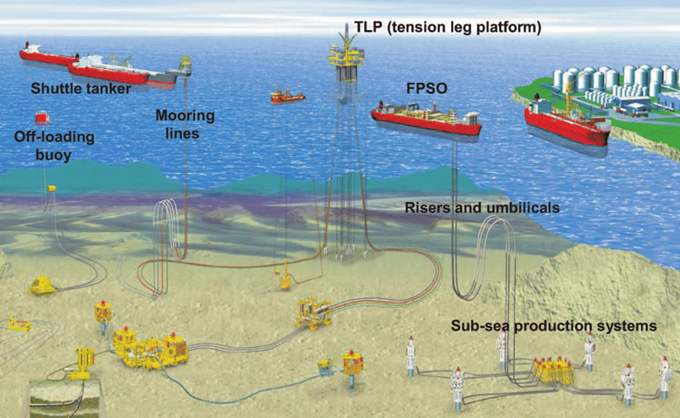
\includegraphics[width=0.9\linewidth]{./Figs/Offshore-production-system.png}
    \caption{Configuração geral esquemática de um sistema offshore de produção. Fonte: elaboração própria, adaptado de Hwang, Roh e Lee (\citeyear{hwang2010fpso}).}
    \label{fig:sistema_offshore}
\end{figure}

Dessa forma, o descomissionamento de sistemas offshore se insere como uma etapa fundamental do ciclo de vida da indústria do petróleo, integrando aspectos técnicos, econômicos, ambientais e regulatórios, que constituem o foco deste trabalho.

\section{Motivação}

Alguns estudos publicados, como \cite{zawawi_environmental_2023}, indicam que um descomissionamento bem-sucedido é caracterizado pela completa vedação do poço, de modo que não haja migração de fluidos pela cabeça do poço nem comunicação entre a formação e o leito marinho através do espaço anular.

No entanto, o descomissionamento não se limita ao abandono seguro de poços. O processo envolve também o desmantelamento de estruturas offshore, com o objetivo de recuperar, sempre que possível, materiais e equipamentos para reutilização ou destinação adequada. Além disso, busca-se a restauração das condições ambientais do leito marinho, de forma a permitir a recomposição da comunidade bentônica a níveis compatíveis com o período anterior às atividades de exploração e produção (E\&P).

No contexto brasileiro, a exploração offshore teve início com a descoberta do campo de Garoupa pela PETROBRAS em 1974, com o poço pioneiro 1-RJS-9A-RJ. A estrutura da plataforma foi instalada em 1979, marcando o início de uma expansão significativa das atividades offshore no país.

Desde então, o avanço tecnológico permitiu a exploração em lâminas d’água progressivamente maiores, resultando na instalação de um volume crescente de estruturas, dutos e equipamentos no leito marinho. Esse crescimento ocorreu em escala superior à observada em fases iniciais da indústria internacional, como no Mar do Norte, onde as lâminas d’água eram significativamente menores.

Como consequência, observa-se atualmente um grande número de instalações com vida útil previamente definida que se aproxima do seu limite operacional. Em alguns casos, essas estruturas já ultrapassaram a vida de projeto originalmente prevista, o que impõe a necessidade de avaliação técnica quanto à continuidade de operação ou à realização do descomissionamento.

Nesse contexto, a decisão entre estender a vida útil de uma instalação offshore ou proceder ao seu descomissionamento torna-se um problema de engenharia que envolve a análise da integridade estrutural, dos riscos associados e das condições operacionais atuais.

\subsection{Critérios técnicos para extensão da vida útil de instalações offshore}

A decisão de estender a vida útil de instalações offshore baseia-se na verificação de que a estrutura continua atendendo aos critérios de segurança e desempenho estabelecidos em normas técnicas. No contexto de estruturas fixas de aço, a ISO 19902:2020 fornece os fundamentos para avaliação da integridade estrutural, ainda que não apresente um procedimento único e explícito para extensão de vida útil. Em vez disso, a norma estabelece critérios de verificação que podem ser aplicados à reavaliação de estruturas existentes \cite{ISO19902_2020}.

A extensão da vida útil está associada ao conceito de \textit{fitness-for-purpose}, no qual se avalia se a instalação permanece apta a operar sob condições reais de carregamento, considerando os efeitos de degradação acumulados ao longo do tempo. Esse processo envolve a análise integrada de diferentes mecanismos de falha.

\subsection{Fadiga estrutural}

A fadiga constitui um dos principais mecanismos limitantes da vida útil de estruturas offshore, em função da ação contínua de carregamentos cíclicos induzidos por ondas, vento e operação. A avaliação do dano acumulado permite estimar a vida remanescente da estrutura, sendo usualmente baseada em modelos como a regra de Palmgren-Miner.

A verificação no estado limite de fadiga (\textit{Fatigue Limit State} -- FLS) é essencial na análise de extensão de vida, uma vez que a propagação de trincas pode comprometer a integridade estrutural ao longo do tempo.

\subsection{Capacidade estrutural e estados limite últimos}

A estrutura deve também atender aos critérios de resistência associados ao estado limite último (\textit{Ultimate Limit State} -- ULS), garantindo sua capacidade de suportar carregamentos extremos. Na reavaliação, considera-se a atualização das ações ambientais e operacionais, bem como possíveis efeitos de degradação.

\subsection{Degradação por corrosão}

A corrosão pode resultar em perda de espessura e redução da capacidade resistente dos elementos estruturais. A avaliação da integridade deve considerar inspeções, medições de espessura e histórico de manutenção.

\subsection{Integridade local e fratura (CTOD)}

Em situações onde são identificadas trincas ou descontinuidades, torna-se necessária a avaliação da integridade local. Nesse contexto, a ISO 19902:2020 apresenta procedimentos para ensaios de CTOD (\textit{Crack Tip Opening Displacement}), utilizados para caracterizar a tenacidade à fratura de materiais e soldas.

A análise baseada em CTOD permite avaliar a capacidade da estrutura de resistir à propagação de trincas sob carregamento, sendo particularmente relevante em regiões soldadas e componentes críticos.

\subsection{Implicações para o descomissionamento}

A extensão da vida útil somente é viável quando a estrutura atende aos critérios de segurança e integridade. Caso esses critérios não sejam satisfeitos, ou quando a manutenção desses níveis de segurança se torna tecnicamente ou economicamente inviável, a alternativa passa a ser o descomissionamento da instalação.

No Brasil, esse processo é regulamentado pela ANP, por meio da Resolução nº 817/2020, que estabelece diretrizes para o abandono de poços e desativação de instalações \cite{ANP_Resolucao_817_2020}.

Assim, a decisão entre estender a vida útil ou proceder ao descomissionamento deve ser entendida como resultado de uma avaliação integrada de natureza estrutural, operacional, econômica e regulatória.

\begin{table}[H]
\centering
\begin{tabular}{ccc}
\toprule
Classe de idade (anos) & Frequência absoluta & Frequência relativa (\%) \\
\midrule
1--6   & 15 & 20,0 \\
7--12  & 20 & 26,7 \\
13--18 & 18 & 24,0 \\
19--24 & 8  & 10,7 \\
25--30 & 4  & 5,3  \\
31--36 & 2  & 2,7  \\
37--43 & 8  & 10,7 \\
\bottomrule
\end{tabular}
\caption{Distribuição das instalações por classes de idade}
\label{tab:classes_idade}
\end{table}

\begin{figure}[H]
  \centering
  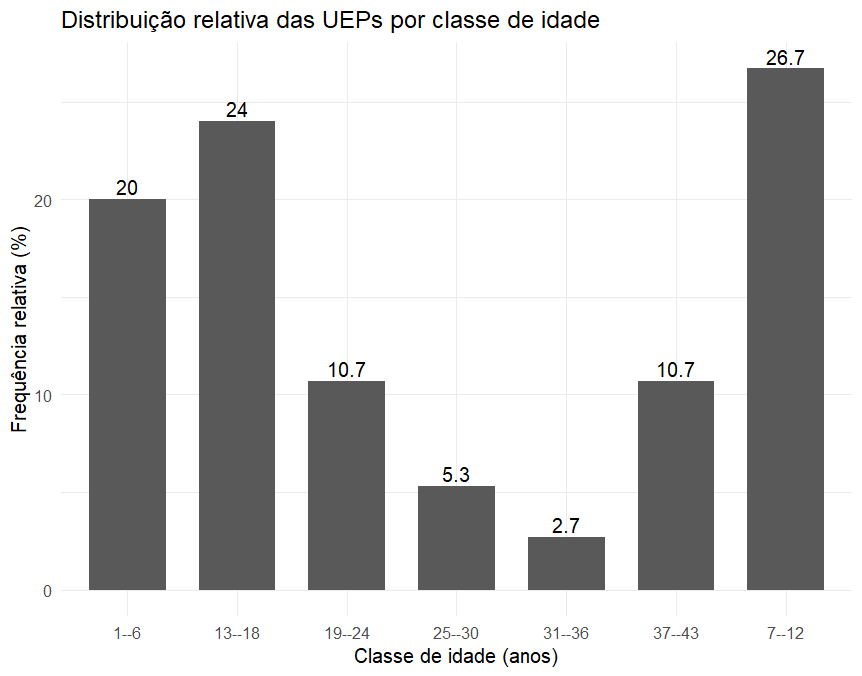
\includegraphics[width=0.9\linewidth]{./Figs/dist_rel_UEP_idade.png}
  \caption{Gráfico das frequências dos tempos de operação}
  \label{fig:dist_rel_UEP_idade}
\end{figure}
\newpage
\printbibliography
\end{document}